% Options for packages loaded elsewhere
\PassOptionsToPackage{unicode}{hyperref}
\PassOptionsToPackage{hyphens}{url}
\documentclass[
]{article}
\usepackage{xcolor}
\usepackage[margin=24mm]{geometry}
\usepackage{amsmath,amssymb}
\setcounter{secnumdepth}{-\maxdimen} % remove section numbering
\usepackage{iftex}
\ifPDFTeX
  \usepackage[T1]{fontenc}
  \usepackage[utf8]{inputenc}
  \usepackage{textcomp} % provide euro and other symbols
\else % if luatex or xetex
  \usepackage{unicode-math} % this also loads fontspec
  \defaultfontfeatures{Scale=MatchLowercase}
  \defaultfontfeatures[\rmfamily]{Ligatures=TeX,Scale=1}
\fi
\usepackage{lmodern}
\ifPDFTeX\else
  % xetex/luatex font selection
\fi
% Use upquote if available, for straight quotes in verbatim environments
\IfFileExists{upquote.sty}{\usepackage{upquote}}{}
\IfFileExists{microtype.sty}{% use microtype if available
  \usepackage[]{microtype}
  \UseMicrotypeSet[protrusion]{basicmath} % disable protrusion for tt fonts
}{}
\makeatletter
\@ifundefined{KOMAClassName}{% if non-KOMA class
  \IfFileExists{parskip.sty}{%
    \usepackage{parskip}
  }{% else
    \setlength{\parindent}{0pt}
    \setlength{\parskip}{6pt plus 2pt minus 1pt}}
}{% if KOMA class
  \KOMAoptions{parskip=half}}
\makeatother
\usepackage{graphicx}
\makeatletter
\newsavebox\pandoc@box
\newcommand*\pandocbounded[1]{% scales image to fit in text height/width
  \sbox\pandoc@box{#1}%
  \Gscale@div\@tempa{\textheight}{\dimexpr\ht\pandoc@box+\dp\pandoc@box\relax}%
  \Gscale@div\@tempb{\linewidth}{\wd\pandoc@box}%
  \ifdim\@tempb\p@<\@tempa\p@\let\@tempa\@tempb\fi% select the smaller of both
  \ifdim\@tempa\p@<\p@\scalebox{\@tempa}{\usebox\pandoc@box}%
  \else\usebox{\pandoc@box}%
  \fi%
}
% Set default figure placement to htbp
\def\fps@figure{htbp}
\makeatother
\setlength{\emergencystretch}{3em} % prevent overfull lines
\providecommand{\tightlist}{%
  \setlength{\itemsep}{0pt}\setlength{\parskip}{0pt}}
\usepackage{mathrsfs}
\usepackage{mathtools}
\DeclareUnicodeCharacter{2212}{\ensuremath{-}}

\DeclareUnicodeCharacter{2265}{\ensuremath{\ge}}
\DeclareUnicodeCharacter{2264}{\ensuremath{\le}}
\DeclareUnicodeCharacter{2295}{\ensuremath{\oplus}}
\DeclareUnicodeCharacter{2297}{\ensuremath{\otimes}}
\DeclareUnicodeCharacter{2208}{\ensuremath{\in}}
\DeclareUnicodeCharacter{2261}{\ensuremath{\equiv}}
\DeclareUnicodeCharacter{21A6}{\ensuremath{\mapsto}}
\DeclareUnicodeCharacter{2192}{\ensuremath{\to}}
\DeclareUnicodeCharacter{03BA}{\ensuremath{\kappa}}
\DeclareUnicodeCharacter{039B}{\ensuremath{\Lambda}}
\DeclareUnicodeCharacter{03C4}{\ensuremath{\tau}}
\DeclareUnicodeCharacter{03A9}{\ensuremath{\Omega}}
\usepackage{bookmark}
\IfFileExists{xurl.sty}{\usepackage{xurl}}{} % add URL line breaks if available
\urlstyle{same}
\hypersetup{
  hidelinks,
  pdfcreator={LaTeX via pandoc}}

\author{}
\date{}

\begin{document}

{
\setcounter{tocdepth}{3}
\tableofcontents
}
\section{The observed infinitesimal collision and the full arithmetic
operator}\label{the-observed-infinitesimal-collision-and-the-full-arithmetic-operator}

22 September 2026. This paper carries the idempotent deformation through
the original observation and then through the determinant, inverse and
marked matrix elements of the full operator. The collision and current
identities are the incoming programme result
\href{https://github.com/KokunoYumeto/zeta-function-research-reader/blob/4ba9285b66af58a6d58fc502a494c1fb45ca5b79/workbenches/splitzero-tandem/continuations/20260922-support-transport/OBSERVED_DEFORMATION_AND_CURRENT.md\#L22}{DF1--12}.
Complete proofs are given below. The full-operator identities OC12--OC17
extend that comparison without removing its Hermitian part or its
original observation. All vector spaces in this paper are finite
dimensional.

\subsection{1. Original metric, observation and retained
parameters}\label{original-metric-observation-and-retained-parameters}

Retain the original data of
\href{https://github.com/KokunoYumeto/zeta-function-research-reader/blob/c9df443d9e1df000dfbb083943f97197e746eb08/workbenches/splitzero-tandem/branches/identity-absorber-square/NATIVE_DUAL_NUMBER_RECEIVER.md}{Native
receiver}, NI1 and NI25--29: \(q=(k+1)^2\), \(k\ge17\),
\(k\equiv1\pmod4\), \(q-1\le N\le2q\), the original source quotient
\((E,G_N)\), original polynomial \(Q_k\), and original surjective
observation \(\Lambda:E\to B\). The source metric and quotient metric
are positive definite. Write \[
Q_B=(\Lambda G_N^{-1}\Lambda^*)^{-1},\quad
L=G_N^{-1}\Lambda^*Q_B,\quad J=LQ_B^{-1/2},\quad P_B=JJ^\dagger.
\tag{OC1}
\] Then \(J^\dagger J=I_B\). Indeed \(L^*G_NL=Q_B\) by multiplying the
displayed matrices, and conjugation by \(Q_B^{-1/2}\) gives the
assertion. Thus \(J\) identifies the Euclidean coordinates on \(B\)
isometrically with the original minimum section; \(P_B\) projects onto
\((\ker\Lambda)^\perp\). A dagger on the source refers to \(G_N\); a
star on observed vectors refers to the Euclidean coordinates in OC1.
Neither operation changes the metric.

The original outgoing source vectors and scalar remain \[
e=b_N/\sqrt{E_N},\quad f=b_{N+1}/\sqrt{F_N},\quad
\epsilon=\sqrt{E_NF_N}/\omega_N>0,
\] \[
M=C+R,\quad C=C^\dagger,\quad R=\epsilon f e^\dagger,
\quad e^\dagger f=0,\quad e^\dagger e=f^\dagger f=1.
\tag{OC2}
\] The complete definitions and proof from the original monic classes
\(b_n=[p_n]\) are NI1--2 and the retained
\href{https://github.com/KokunoYumeto/zeta-function-research-reader/blob/c9df443d9e1df000dfbb083943f97197e746eb08/workbenches/splitzero-tandem/branches/identity-absorber-square/sources/OBSERVED_CURRENT_PLANE.tex}{OCP
source}, OCP5--7. Put \[
P_e=ee^\dagger,\quad \Pi=ee^\dagger+ff^\dagger,\quad
F(s)=R+sP_e,\quad M(s)=C+F(s).
\] Since \(R^2=P_eR=0\), \(RP_e=R\), and \(P_e^2=P_e\), multiplication
gives \(F(s)^2=sF(s)\). The original arithmetic action is precisely
\(M(0)\); the entire displayed family is an actual family of operators
on its unchanged metric space.

Define \[
u=J^\dagger e,\quad v=J^\dagger f,\quad U=[u,v],\quad
\mathcal C=U^*U=\begin{pmatrix}a&r\\\bar r&d\end{pmatrix},
\quad \Delta=ad-|r|^2>0.
\tag{OC3}
\] Here \(a=u^*u\), \(r=u^*v\), \(d=v^*v\), and
\(0\prec\mathcal C\preceq I_2\) are the original measured columns and
finite area assertion
\href{https://github.com/KokunoYumeto/zeta-function-research-reader/blob/4ba9285b66af58a6d58fc502a494c1fb45ca5b79/workbenches/splitzero-tandem/continuations/20260922-support-transport/SUPPORT_SPECTRUM_AND_TERMINAL_MASS.md\#L44}{ST5--6}.
We retain this proved domain. In particular \(a>0\), and \(u,v\) are
independent. Their measured support is \(A=UU^*\), while the orthogonal
range projection is \[
P=U\mathcal C^{-1}U^*.
\tag{OC4}
\] The inverse exists by \(\Delta>0\). Direct multiplication proves
\(P^2=P=P^*\); it fixes both columns and vanishes on their orthogonal
complement. No identification of \(A\), \(P\), \(\Pi\), or \(P_B\) is
made. Their exact compression relation is
\(A-A^2=J^\dagger\Pi(I-P_B)\Pi J\), obtained by expanding both sides.

\subsection{2. The shifted family and its exact
algebra}\label{the-shifted-family-and-its-exact-algebra}

Put \(C_B=J^\dagger CJ=C_B^*\). Then \[
F_B(s)=J^\dagger F(s)J=(\epsilon v+su)u^*,\quad
M_B(s)=C_B+F_B(s),\quad \lambda(s)=as+\epsilon r.
\tag{OC5}
\] The identity \(u^*(\epsilon v+su)=\lambda(s)\) proves \[
F_B(s)^2=\lambda(s)F_B(s),\qquad
J^\dagger F(s)(I-P_B)F(s)J=(s-\lambda(s))F_B(s).
\tag{OC6}
\] For the second formula subtract \(F_B(s)^2\) from
\(J^\dagger F(s)^2J=sF_B(s)\). This retains the exact contribution
through the original hidden source kernel.

An explicitly proved orthonormal frame of \(\operatorname{im}P\) is \[
g=u/\sqrt a,\qquad h=\frac{v-(r/a)u}{\sqrt{\Delta/a}},\qquad b=\epsilon\sqrt\Delta>0.
\] The numerator of \(h\) is orthogonal to \(u\) and has squared norm
\(d-|r|^2/a=\Delta/a\). In this frame, \[
F_B(s)=\begin{pmatrix}\lambda(s)&0\\b&0\end{pmatrix}
\quad\text{on }\operatorname{im}P,
\qquad F_B(s)|_{\ker P}=0.
\tag{OC7}
\] Thus the homomorphism \[
\mathcal A_B=\mathbb C[s,z]/(z(z-\lambda(s)))
\longrightarrow\operatorname{End}(B)\otimes\mathbb C[s],
\quad 1\mapsto I_B,\ z\mapsto F_B(s)
\tag{OC8}
\] is injective. Monic division reduces a kernel element to
\(A(s)+B(s)z\); applying it to \(h\) gives \(A=0\), and the
\(h\)-coefficient after applying it to \(g\) gives \(bB=0\), hence
\(B=0\). It is an isomorphism onto the generated algebra and is free of
rank two over \(\mathbb C[s]\). The supported version sends \(1\) to
\(P\). The exact affine base isomorphism with the original family is
\(t=as+\epsilon r\), with inverse \(s=(t-\epsilon r)/a\), and leaves the
generator \(z\) unchanged.

The fibre at \[
s_*=-\epsilon r/a
\quad\text{has}\quad
\widetilde R=F_B(s_*)=\epsilon v u^*-(\epsilon r/a)uu^*=b h g^*,
\quad \widetilde R^2=0\ne\widetilde R.
\tag{OC9}
\] Consequently
\(\mathbb C[\eta]/\eta^2\to\mathbb C[I_B,\widetilde R]\),
\(\eta\mapsto\widetilde R\), is a faithful isomorphism by the
independence proof in OC8. At \(s\ne s_*\), evaluation at
\(z=0,\lambda(s)\) gives the fibre isomorphism with
\(\mathbb C\times\mathbb C\), with inverse
\((c_0,c_1)\mapsto c_0(1-z/\lambda)+c_1z/\lambda\). The two eigenline
modules are \(\mathbb C[s]h\) and \(\mathbb C[s](\lambda g+bh)\). Their
sum is \(\mathbb C[s]h+\lambda\mathbb C[s]g\), so its cokernel in the
plane is exactly \(\mathbb C[s]/(s-s_*)\), through
\(Ag+Bh\mapsto A\bmod(s-s_*)\). This is the module specified by failure
of the eigenlines to span at collision.

For \(s\ne s_*\), put \(E_1=F_B(s)/\lambda(s)\), \(E_0=P-E_1\). Their
exact norms and the continuity of the original family are \[
\|E_1\|=\|E_0\|=\sqrt{1+\frac{b^2}{|as+\epsilon r|^2}},
\qquad \|F_B(s)-F_B(s_*)\|=a|s-s_*|.
\tag{OC10}
\] In OC7 the nonzero column of \(E_1\) is \((1,b/\lambda)^T\), and the
nonzero row of \(E_0\) is \((-b/\lambda,1)\). Their Euclidean lengths
prove the first assertion. The second is the norm of \((s-s_*)uu^*\),
and \(\|uu^*\|=a\).

\subsection{3. The signed current is a coordinate of the
collision}\label{the-signed-current-is-a-coordinate-of-the-collision}

Set \(\omega(s)=\Im\lambda(s)\). The original full observed current is
\[
W_B(s)=i(M_B(s)-M_B(s)^*)=W_B(0)-2\Im(s)uu^*,
\] \[
W_B(s)|_{g,h}=\begin{pmatrix}-2\omega(s)&-ib\\ib&0\end{pmatrix},
\quad \operatorname{tr}W_B(s)=-2\omega(s),
\quad \det(W_B(s)|_{g,h})=-b^2.
\tag{OC11}
\] The Hermitian \(C_B\) cancels in the difference, while the orthogonal
complement of the plane remains in its kernel. The determinant
calculation proves rank two for every \(s\). At \(s=0\),
\(\operatorname{tr}W_B(0)=-2\epsilon\Im r\), hence \[
\Im s_*=\frac{\operatorname{tr}W_B(0)}{2a},\qquad
W_B(s_*)-W_B(0)=2\epsilon\Im r\,gg^*.
\] Therefore the collision lies on the real path exactly when the
original current trace vanishes. Every real parameter leaves the
complete current unchanged. For a fixed marked vector
\(y=c_g g+c_hh+y_\perp\), its exact signed values are \[
y^*W_B(0)y=2b\Im(\bar c_g c_h)-2\epsilon\Im r\,|c_g|^2,
\quad y^*W_B(s_*)y=2b\Im(\bar c_g c_h).
\] This proves the rank-one correction for the marked bound; it
preserves the phase of both components. Detailed sharp support
inequalities and their module receivers are developed in
\href{https://github.com/KokunoYumeto/zeta-function-research-reader/blob/c9df443d9e1df000dfbb083943f97197e746eb08/workbenches/splitzero-tandem/branches/identity-absorber-square/OBSERVED_SUPPORT_PROPAGATION.md}{Observed
support propagation}.

\subsection{4. Pullback through the determinant and resolvent of the
whole
operator}\label{pullback-through-the-determinant-and-resolvent-of-the-whole-operator}

The full \(C_B\) remains in every formula of this section. For any
parameters \(s,t\in\mathbb C\), \[
M_B(s)=M_B(t)+(s-t)uu^*.
\tag{OC12}
\] For an independent spectral coordinate \(\zeta\), set \[
p_t(\zeta)=\det(\zeta I_B-M_B(t)),\qquad
q_t(\zeta)=u^*\operatorname{adj}(\zeta I_B-M_B(t))u.
\] Then, as an identity of polynomials in \(s,t,\zeta\), \[
\boxed{p_s(\zeta)=p_t(\zeta)-(s-t)q_t(\zeta),\qquad q_s(\zeta)=q_t(\zeta).}
\tag{OC13}
\] For completeness, column multilinearity proves
\(\det(H-\xi uu^*)=\det H-\xi u^*\operatorname{adj}(H)u\): every term
selecting two perturbation columns vanishes because they are multiples
of the same vector; the single-column terms are the cofactor expansion.
This proves the first formula without any invertibility hypothesis.
Apply it with another independent parameter \(s+\xi\), once based at
\(s\) and once at \(t\); equality of the coefficients of \(\xi\) proves
the second. In particular \[
p_*(\zeta)=p_0(\zeta)-s_*q_0(\zeta).
\] Thus the exact additional datum that propagates the full
characteristic polynomial is the polynomial \(q_0\), including its
dependence on \(C_B\) and the original vector \(u\). It can be computed
from the original adjugate even at an eigenvalue.

Now let \(p_t(\zeta)\ne0\), and define \[
G_t(\zeta)=(\zeta I_B-M_B(t))^{-1},\quad
m_t(\zeta)=u^*G_t(\zeta)u.
\] OC13 gives \(p_s/p_t=1-(s-t)m_t\). Consequently the inverse at \(s\)
exists exactly when this scalar is nonzero, and then \[
\boxed{G_s=G_t+
\frac{(s-t)G_tu u^*G_t}{1-(s-t)m_t},\qquad
m_s=\frac{m_t}{1-(s-t)m_t}.}
\tag{OC14}
\] Multiply the proposed inverse by \(\zeta I-M_B(t)-(s-t)uu^*\) on
either side. The two rank-one terms cancel because their remaining
coefficient is \((s-t)/(1-(s-t)m_t)-(s-t)-(s-t)^2m_t/(1-(s-t)m_t)=0\).
This proves the inverse formula. Multiplication by \(u^*\) and \(u\)
gives the scalar formula. No commutation of \(C_B\) with \(P\) or
\(uu^*\) is required.

Every pair of original marked vectors \(x,y\in B\) therefore has the
exact receiver \[
x^*G_s y=x^*G_t y+
\frac{(s-t)(x^*G_tu)(u^*G_ty)}{1-(s-t)m_t}.
\tag{OC15}
\] This follows by applying the two linear functionals to OC14. The two
factors retain their separate order and complex phases. The exact norm
of the inverse difference is \[
\boxed{\|G_s-G_t\|=
\frac{|s-t|\,\|G_tu\|\,\|G_t^*u\|}{|1-(s-t)m_t|}.}
\tag{OC16}
\] Indeed \(G_tu u^*G_t=(G_tu)(G_t^*u)^*\), whose rank-one norm is the
product of the two vector norms: Cauchy--Schwarz proves the upper bound
and a unit vector parallel to \(G_t^*u\) attains it. These vectors are
nonzero because \(G_t\) is invertible and \(u\ne0\). OC16 gives a sharp
perturbation identity wherever both inverses exist, including \(s=s_*\).

The scalar obstruction itself defines an exact spectral alternative. At
\(\zeta\) in the resolvent of \(M_B(t)\), if \(1-(s-t)m_t=0\), then
\(s-t\ne0\), \(m_t\ne0\), and \[
\ker(\zeta I-M_B(s))=\mathbb C G_tu.
\tag{OC17}
\] The vector \(G_tu\) lies in the kernel by direct multiplication.
Conversely, any kernel vector satisfies \(x=(s-t)G_tu(u^*x)\), so it
belongs to this line. The corresponding left kernel is
\(\mathbb C u^*G_t\). This constructs the precise eigenspace exposed by
the failed inverse. Algebraic multiplicity remains determined by the
order of the zero in the explicit polynomial OC13; no assertion of
simplicity replaces that calculation.

\subsection{5. Consequence maps and source
identity}\label{consequence-maps-and-source-identity}

The propagation now has explicit domains and codomains: the original
family \(\mathbb C[t,z]/z(z-t)\) pulls back by \(t=as+\epsilon r\) to
OC8; its collision quotient is the faithful dual-number algebra OC9;
OC11 returns its displacement to the original signed current; and
OC13--OC17 return the same displacement to the characteristic
polynomial, inverse, marked inverse pairings and eigenspace of the full
\(M_B\). The retained support and cotangent/Frobenius receivers appear
in the accompanying papers. No evaluation of a native arithmetic period,
new RH bound, or quantum-group positivity theorem is asserted by these
finite identities.

Source provenance: OC5--OC11 rederive DF1--12 of the public programme
proof cited above, using the complete native definitions NI1 and
NI25--29. The determinant calculation in OC13 is proved directly by
multilinearity; the rank-one inverse calculation in OC14 is proved
directly by multiplication. Both are standard linear-algebra
constructions, here applied with every original programme parameter
retained. Their availability does not establish historical novelty of
rank-one perturbation theory.

\begin{figure}
\centering
\pandocbounded{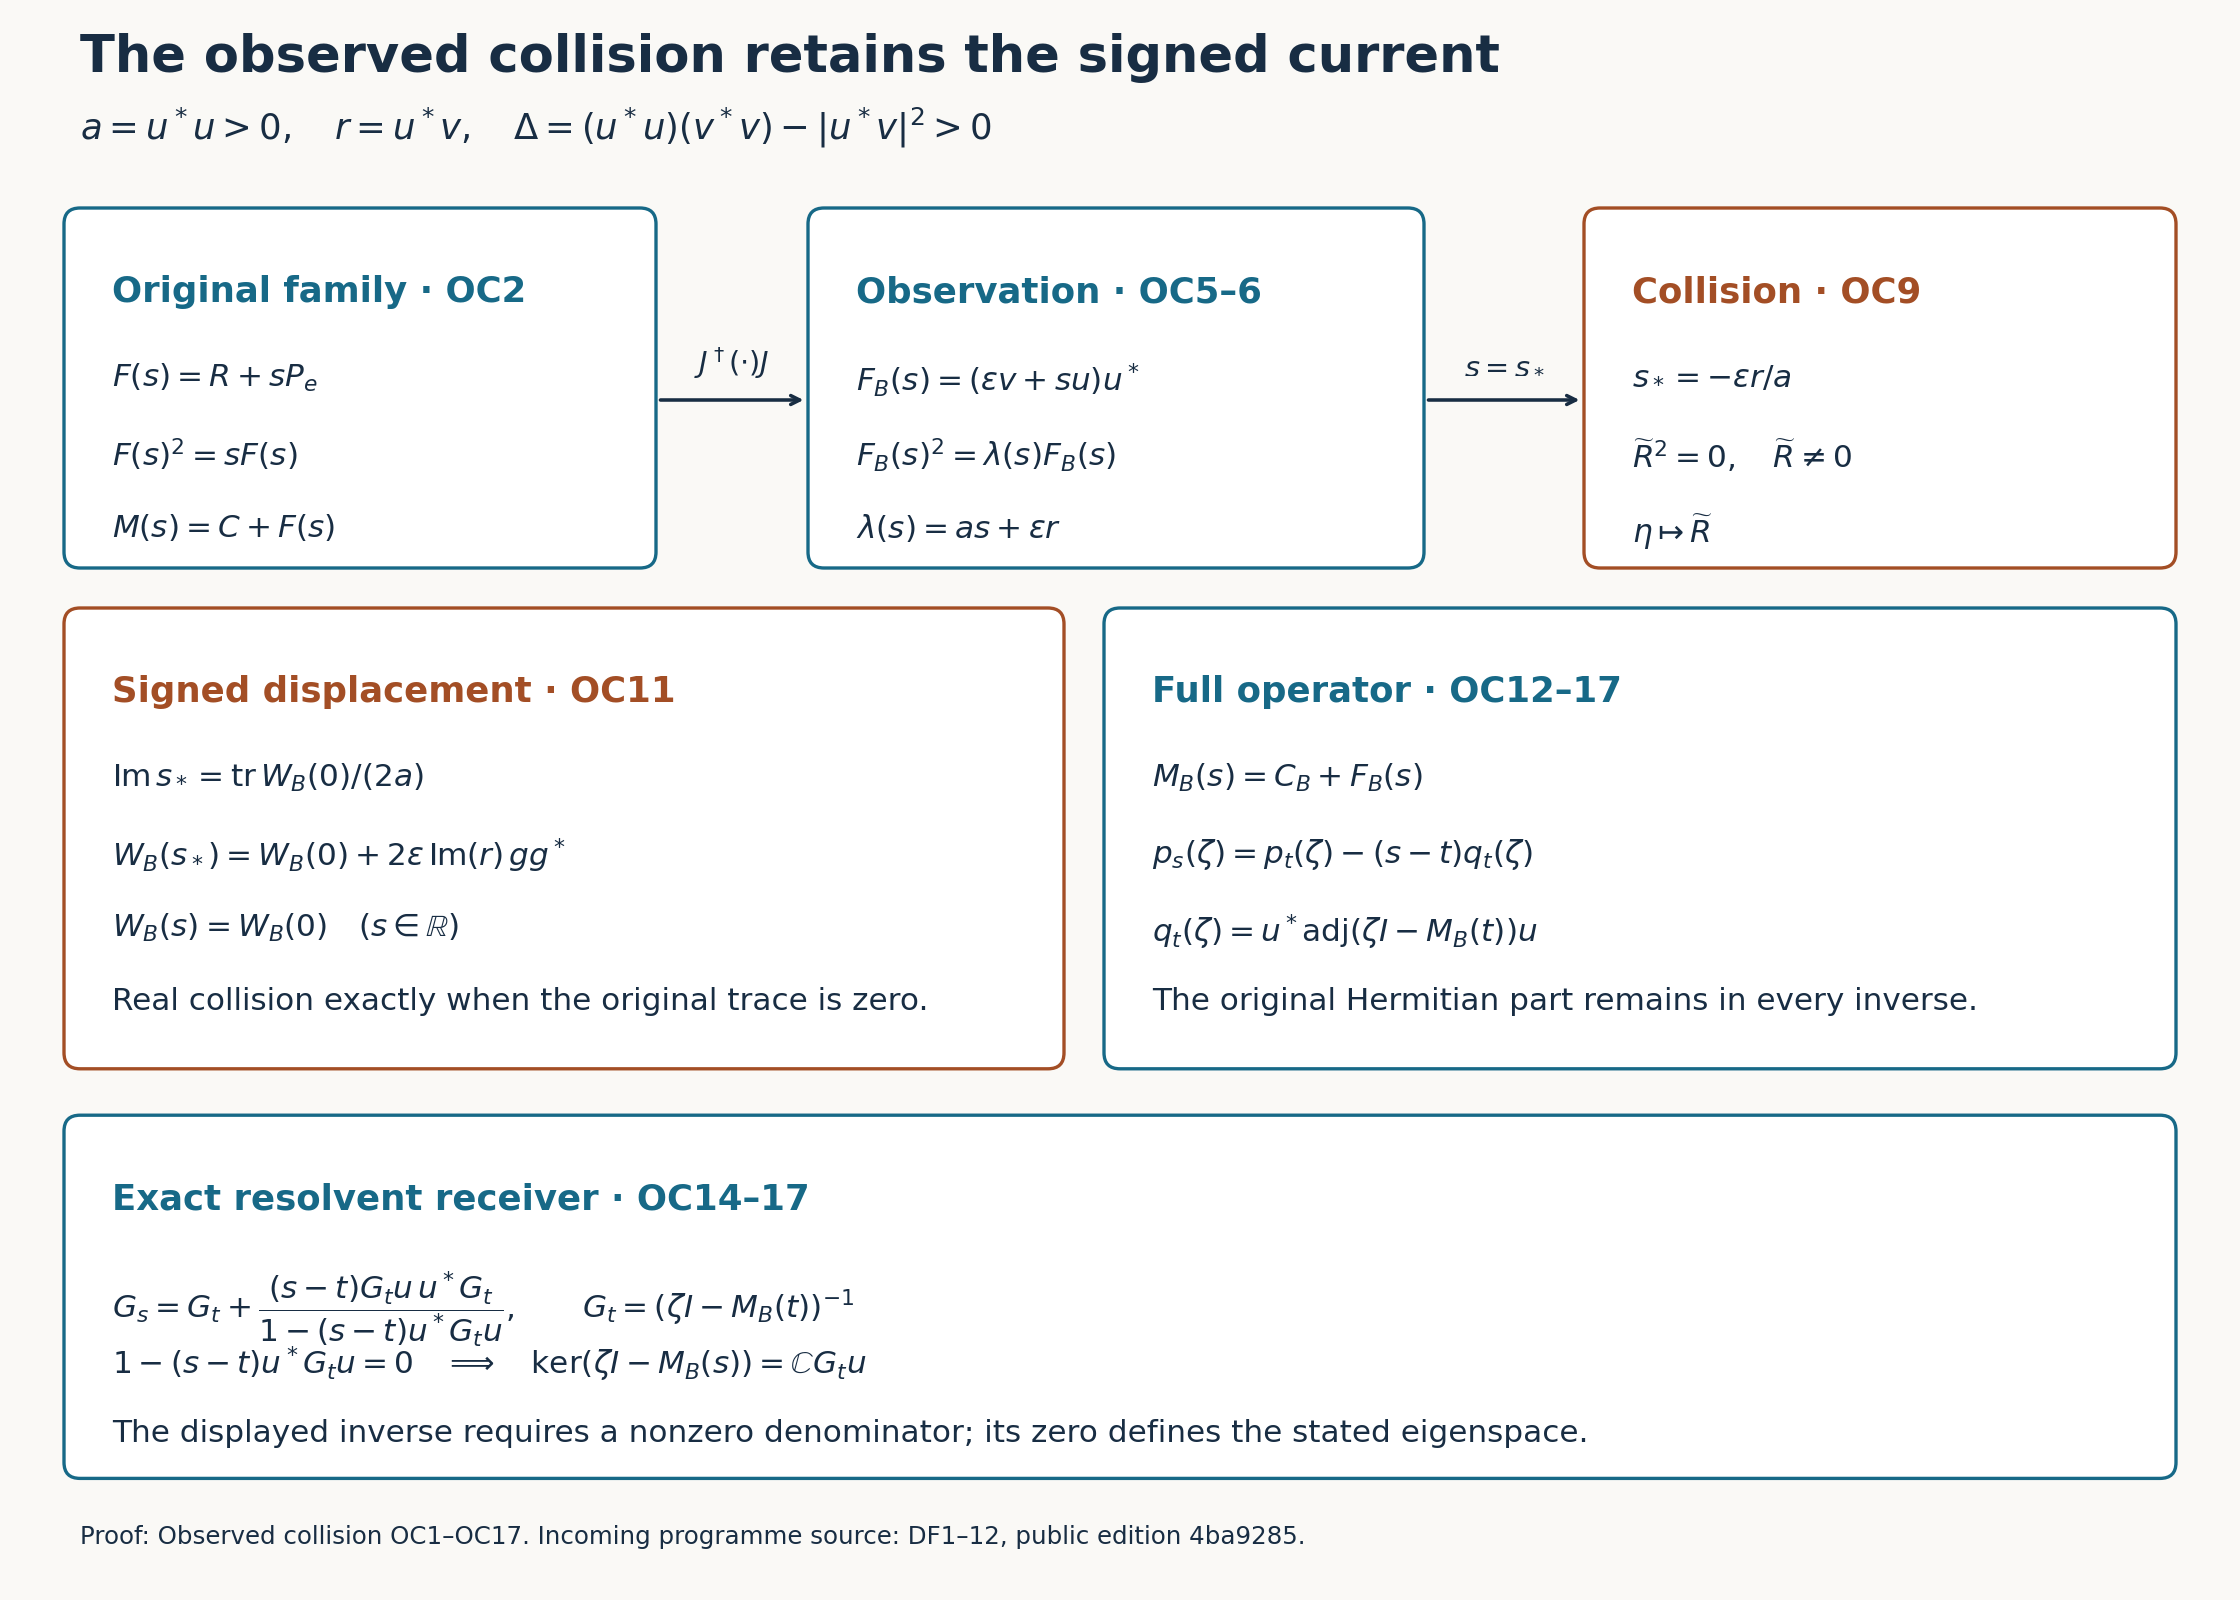
\includegraphics[keepaspectratio,alt={Shifted collision, the original current trace and the exact full-operator receiver}]{figures/18_observed_collision.png}}
\caption{Shifted collision, the original current trace and the exact
full-operator receiver}
\end{figure}

The figure displays the affine parameter map and the complex collision
point symbolically. Its signed imaginary coordinate is exactly OC11. The
determinant and resolvent arrows are OC13--OC17. It is a diagram of the
proved maps, not a numerical evaluation of the original period.

\end{document}
